\documentclass[tikz,border=10pt]{standalone}
\begin{document}
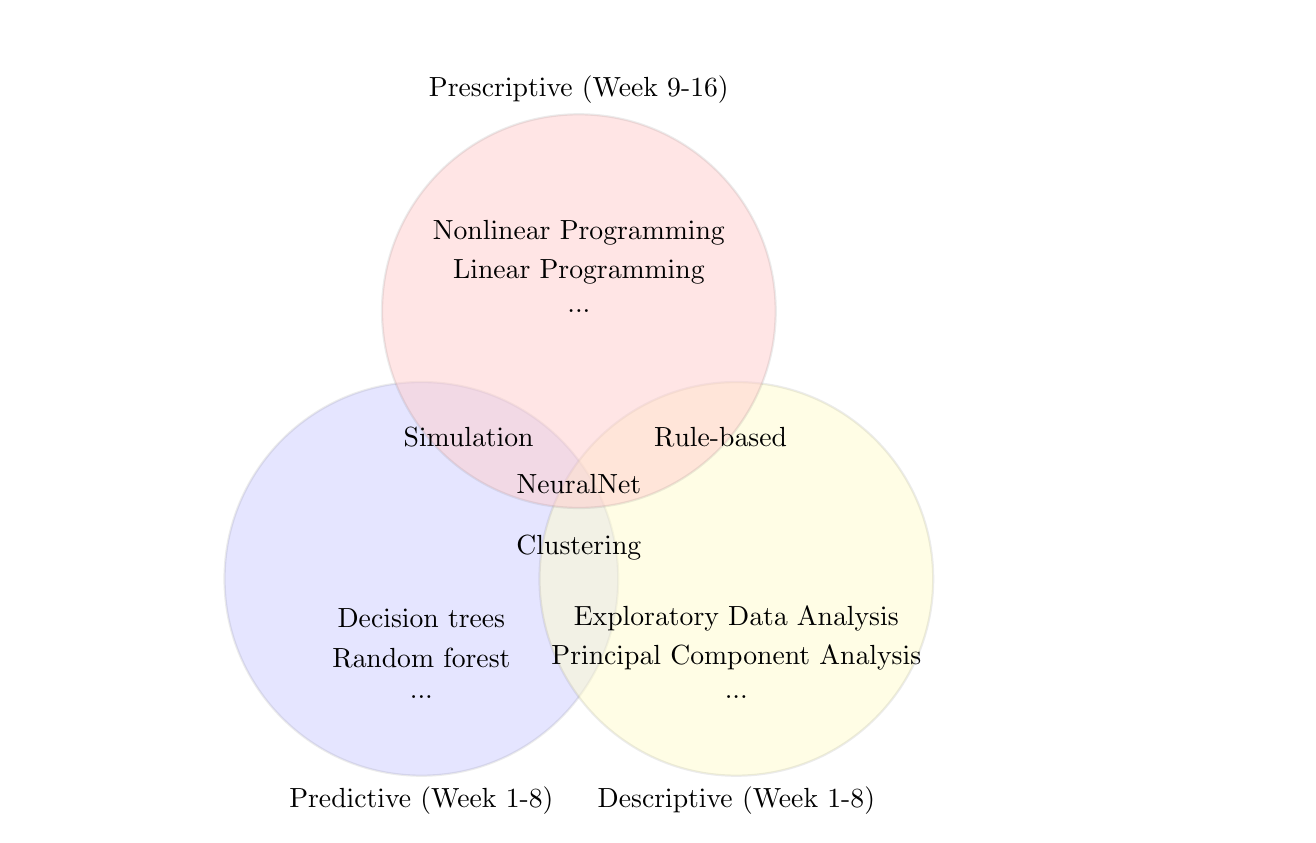
\begin{tikzpicture}[>=stealth, node distance=4cm, auto]
    \useasboundingbox (-1, -3) rectangle (15, 7);
    
    % Define styles
    \tikzstyle{pred}=[circle, thick, draw=black!75, fill=blue!20, minimum size=50mm, align=center, label=below:, draw opacity=0.1, fill opacity=0.5]
    \tikzstyle{pres}=[circle, thick, draw=black!75, fill=red!20, minimum size=50mm, align=center, label=below:, draw opacity=0.1, fill opacity=0.5]
    \tikzstyle{desc}=[circle, thick, draw=black!75, fill=yellow!20, minimum size=50mm, align=center, label=below:, draw opacity=0.1, fill opacity=0.5]

    \node[pred, label=below:Predictive (Week 1-8)] (A) at (4,0) {};    
    \node[desc, label=below:Descriptive (Week 1-8)] (C) at (8,0) {};
    \node[pres, label=above:Prescriptive (Week 9-16)] (B) at (6,3.4) {};

    \node at (4,-0.5) {Decision trees};
    \node at (4,-1) {Random forest};
    \node at (4,-1.5) {...};

    \node at (6,3.9) {Linear Programming};
    \node at (6,4.4) {Nonlinear Programming};
    \node at (6,3.4) {...};

    \node at (8,-0.5) {Exploratory Data Analysis};
    \node at (8,-1) {Principal Component Analysis};
    \node at (8,-1.5) {...};

    \node at (6,1.2) {NeuralNet};
    \node at (7.8,1.8) {Rule-based};
    \node at (4.6,1.8) {Simulation};
    \node at (6,0.4) {Clustering};
\end{tikzpicture}
\end{document} 